\documentclass[12pt]{article}
\usepackage{graphicx} % Required for inserting images
\usepackage{blindtext}
\usepackage{titlesec}
\usepackage[a4paper]{geometry}
\geometry{   % AS PER PG MANUAL
  top=3cm,
  bottom=3cm,
  left=4cm,
  right=2cm,
}
\usepackage{colortbl}
\usepackage[table]{xcolor}
\usepackage{graphicx}
\usepackage{subfigure}
\usepackage{textcomp}
\usepackage{float}
\usepackage{natbib}
\usepackage{afterpage}
\usepackage{fancyhdr}

\pagestyle{fancy}
\fancyhf{}
\rhead{\thepage}   % TO PUT PAGE NUMBER AT TOP RIGHT AS PER REQUIRED IN MANUAL
\renewcommand{\headrulewidth}{0pt}

% \usepackage[style=authoryear-ibid,backend=biber]{biblatex}
% \addbibresource{reference.bib}% Syntax for version >= 1.2
\linespread{1.5}
\usepackage{newtxtext,newtxmath}

\usepackage{titlesec}
\titleformat{\section}{\normalfont\Large\bfseries\centering}{\thesection}{1em}{}


\begin{document}


%%%%%%%%%%%%%%%%%%%%%%%%%%%%%%%%%%%%%%%%%%%%%%%%%%%%%
% HERE STARTS YOUR COVER PAGE
%%%%%%%%%%%%%%%%%%%%%%%%%%%%%%%%%%%%%%%%%%%%%%%%%%%%%%
% Cover Page with Different Geometry
\newgeometry{top=4cm, bottom=4cm, left=4cm, right=2cm
}
\begin{titlepage}
    % Your cover page content goes here
\begin{center}
   \section*{\fontsize{24}{24}\selectfont MY THESIS TITLE IN CAPITAL LETTERS}
   
%    %\vspace{1cm}
% \textbf{Pore pressure prediction from well data of Mahanadi basin using various machine learning algorithms}
% \vspace{1cm}

\textbf{BY}

\textbf{\fontsize{14}{16}\selectfont MY NAME}
% \vspace{1cm}

\textbf{\fontsize{14}{16}\selectfont (Admission No. XXXXXXX)}


\begin{figure}[H]
    \centering
    
\includegraphics[width=4cm]{ismlogo.jpg}
   
    \label{fig:enter-labe2l}
\end{figure}

\textbf{\fontsize{14}{16}\selectfont THESIS\\ SUBMITTED TO\\
DEPARTMENT OF APPLIED GEOPHYSICS\\
INDIAN INSTITUTE OF TECHNOLOGY\\
(INDIAN SCHOOL OF MINES), DHANBAD\\}


\vspace{1cm}

\textbf{\fontsize{14}{16}\selectfont For the award of the degree of\\
MASTER OF SCIENCE \& TECHNOLOGY\\   %% YOUR DEGREE NAME HERE
NOVEMBER 2023}

\end{center}

\end{titlepage}
\restoregeometry % Restore the default geometry

%%%%%%%%%%%%%%%%%%%%%%%%%%%%%%%%%%%%%%%%%%%%%%%%
% COVER PAGE ENDS
%%%%%%%%%%%%%%%%%%%%%%%%%%%%%%%%%%%%%%%%%%%%%%%%

\newpage
\clearpage 
\setcounter{page}{1}  % PAGE NUMBER FROM WHERE YOU WANT TO START PAGE NUMBERING 

%%%%%%%%%%%%%%%%%%%%%%%%%%%%%%%%%%%%%%%%%%%%%%%

\section*{ACKNOWLEDGEMENT}
I extend my sincere gratitude to Prof.AA, a distinguished Professor in the Department of BB at IIT(ISM) Dhanbad. 

MIND THAT YOU NEED SOME CERTIFICATES BEFORE THE ACKNOLEGMENT. REFER PG MANUAL ON IIT ISM SITE FOR CERTIFICATES. 
THIS TEMPLATE IS AS PER REQUIREMNT OF YEAR 2023-2024 BATCH. PLEASE MAKE CHANGES FOR YOURSELF IF THINGS CHANGES LATER.


\newpage
\section*{CONTENTS}
\begin{tabular}{ccc}

 Abstract  &  .........                  &  5 \\
CHAPTER 1  & Introduction                &  6 \\
CHAPTER 2  &  Data                       &  9 \\
CHAPTER 3  & Method                      &  13 \\
CHAPTER 4  & Your Chapter Title Goes Here   &  17 \\
CHAPTER 5  &  Summary and Conclusions    &  21 \\
References & .........                   & 31

\end{tabular}

\newpage
\section*{}
\listoftables


\section*{}
\listoffigures

\newpage
\section*{Abstract}
Could you write your ABSTRACT here?

\newpage
\section*{CHAPTER 1 \\Introduction}

This is an introduction chapter. You should put citations like this \citep{Zhang2011}.

If you need points in it- 

\begin{enumerate}
    \item Random Forest (RF)
    \item  Gradient Boosting
    \item Convolutional neural network (CNN)
    \item Long Short-term Memory (LSTM)

\end{enumerate}


\newpage
\section*{CHAPTER 2\\Data}
The speed of light is approximately 299,792,458 meters per second, making it the fastest-known phenomenon in the universe.

Getting figure here- 

\begin{figure}[H]
    \centering
    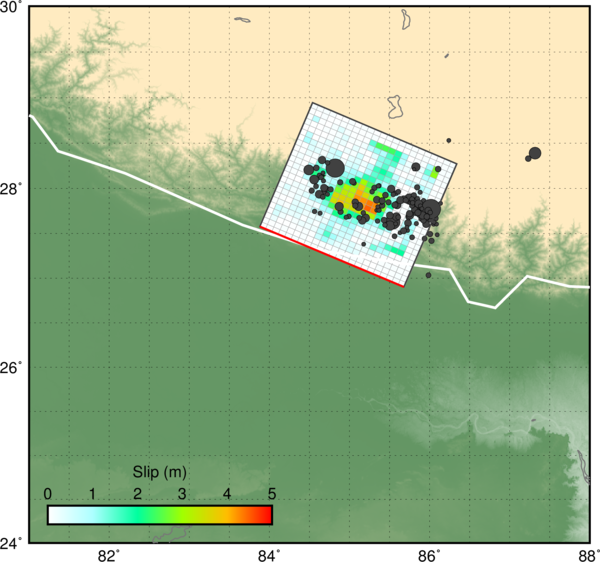
\includegraphics[width=\textwidth]{basemap.png}
    \caption{ caption your map}
    \label{fig:well}
\end{figure}


\newpage
\section*{CHAPTER 3\\ Method }

Total internal reflection is a phenomenon in optics where light, when traveling from a denser medium to a less dense medium at an angle greater than the critical angle, reflects back into the denser medium rather than refracting out. 

\subsection*{My subsection}

This principle is the basis for optical fibers used in telecommunications.

\newpage
\section*{CHAPTER 4\\Your Chapter Title Goes Here }

Distributed Acoustic Sensing (DAS) is a transformative technology in geosciences and engineering. DAS records ground motion along fiber-optic cables that are comparable to those obtained by single-component accelerometers or geophones. The transformative potential arises from the fiber itself being the sensor and allowing for a spatially continuous measurement. The fiber can be tens of kilometers in length and it can be located in shallowly buried trenches, in boreholes, or in some combination. The fiber geometry can encompass a large volume that can be tens of cubic kilometers in size. DAS inherently possesses properties of a large-N seismic array. The rapidly increasing interest in DAS arises from its potential to be used in continuous arrays that are kilometers in length while providing spatial resolution of meters and frequency response from millihertz to kilohertz.

DAS applications in geosciences and engineering are numerous and growing including opportunities for deploying early warning systems for earthquakes, volcanic eruptions, continental and marine landslides, and avalanches, and for monitoring reservoirs and civil infrastructure. DAS can complement and supplement conventional seismic sensors and arrays already used across a wide range of disciplines.

\subsection*{Statistical Analysis}

YOUR EQUATIONS GOES GOOD

The error between predicted and actual pore pressure has been calculated as \( R^2 \) coefficient. The Coefficient of Determination  \( R^2 \), indicates the goodness of fit of the regression line to the actual data points.

 \( R^2 \) ranges from 0 to 1, where:
 

1. Sum of Squares Total (SST):

   \[ SST = \sum_{i=1}^{n} (y_i - \bar{y})^2 \]

2. Sum of Squares Regression (SSR):

   \[ SSR = \sum_{i=1}^{n} (\hat{y}_i - \bar{y})^2 \]

\newpage
\section*{CHAPTER 5\\Summary and Conclusions}

I WANT SUBPLOTS IN MY FIGURE. 

\begin{figure}[H]
    \centering
    \subfigure[ONE]{
        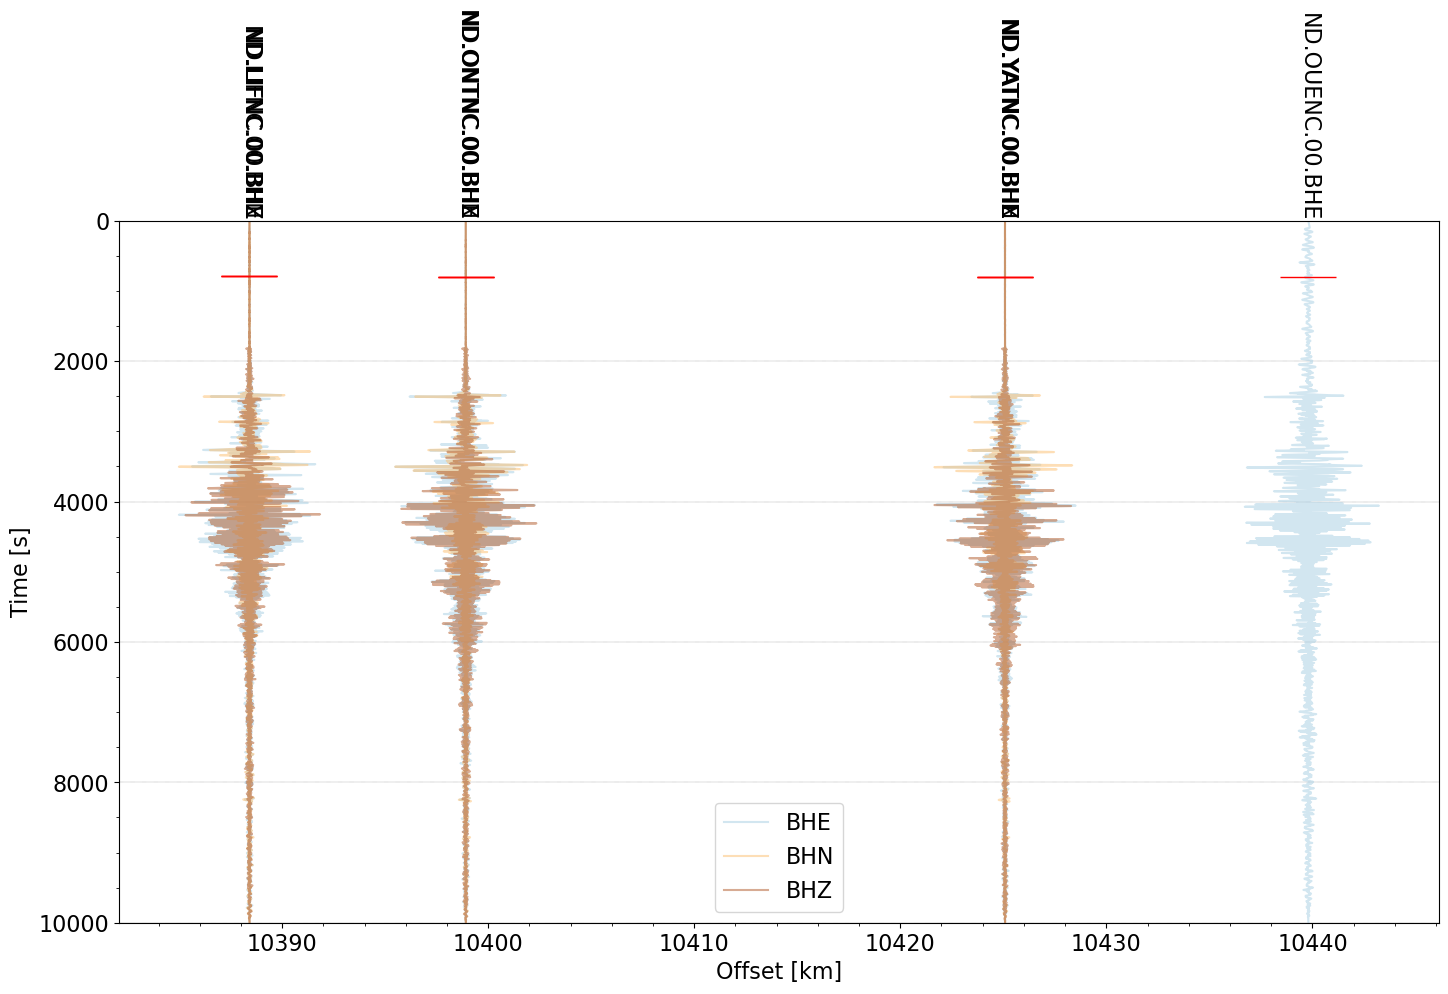
\includegraphics[width=0.5\linewidth]{my_pic.png} % Include your first plot
        \label{fig:plot1}
    }
    \hfill
    \subfigure[TWO ]{
        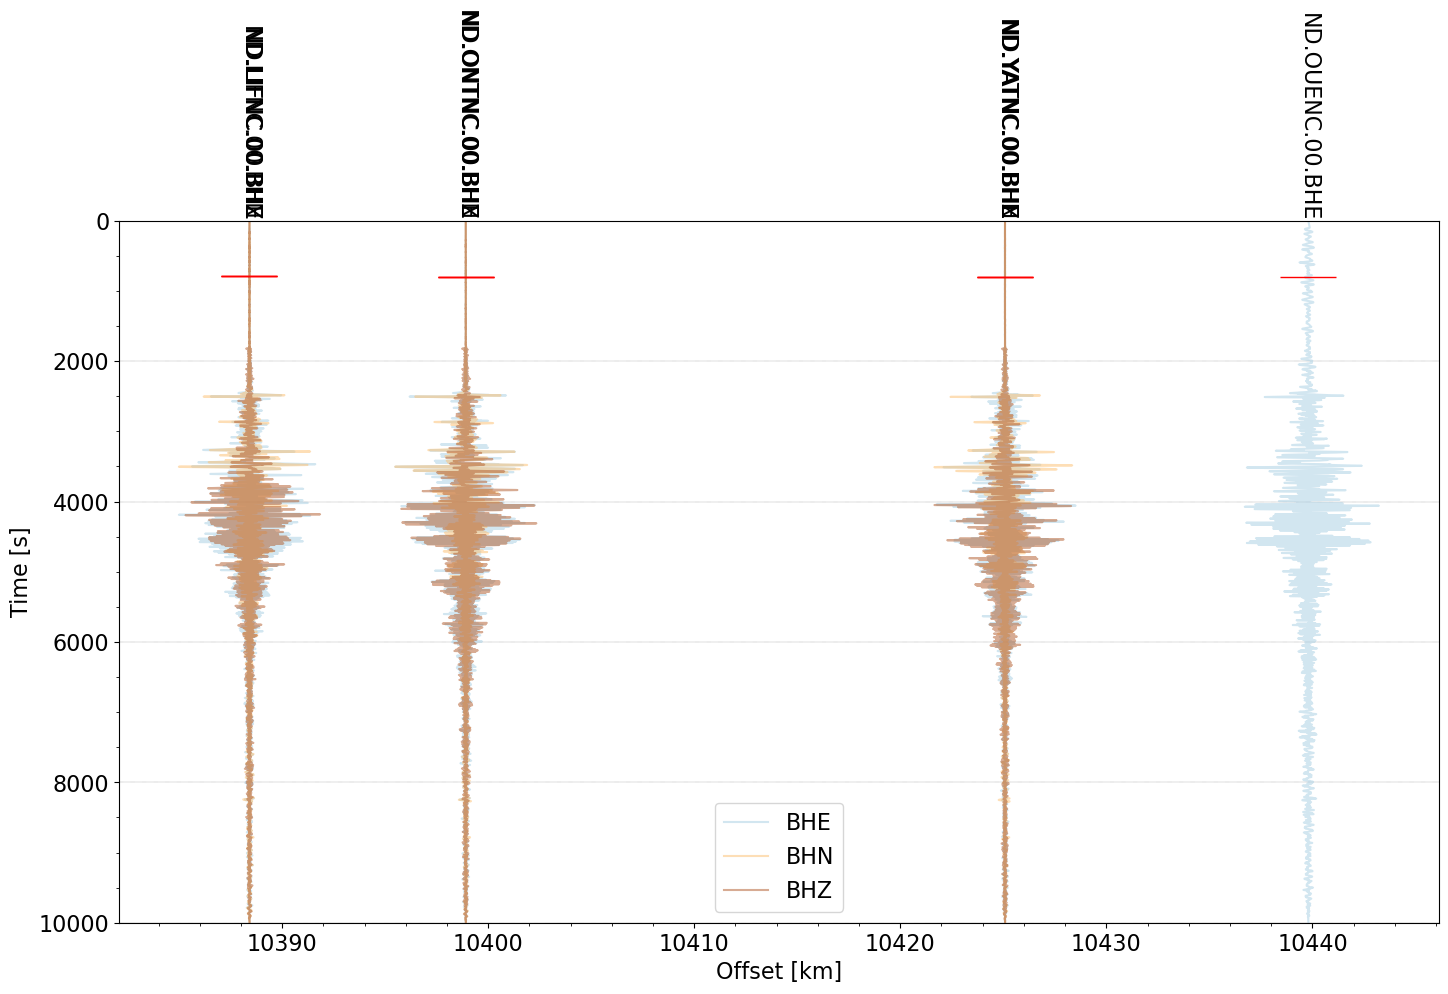
\includegraphics[width=0.5\linewidth]{my_pic.png} % Include your second plot
        \label{fig:plot2}
    }
    \caption{CAPTIONS}
    \label{fig:two_plots}
\end{figure}

%  \input{table}  % if you need to put some tables

\newpage
\subsection*{Conclusions}
As we wrap up this discussion, I hope this template helps you save your time doing formatting.


\newpage

\bibliographystyle{apalike}  %Harvard style reference 
\bibliography{reference}

\end{document}
